\documentclass{article} % Класс печатного документа

% для поддержки русского языка
\usepackage[T2A]{fontenc} % поддержка специальных русских символов
\usepackage[utf8]{inputenc} % Кодировка исходного текста - utf8
\usepackage[english,russian]{babel} % Поддержка языка - русского с английским
\usepackage{indentfirst} % Отступ в первом абзаце

\usepackage{graphicx} % Для вставки картинок
\usepackage{hyperref} % Для вставки гиперссылок
\usepackage{listings} % Для вставки кусков кода
\usepackage{float} % Для точного позиционирования картинок
\usepackage{amsmath} % Для отключения нумерации у указанных формул
\usepackage{listings} % Добавление листингов
\usepackage[justification=centering]{caption} % для центрирования подписи к таблице

\title{Отчёт 6\\
Логистическая регрессия} % заголовок документа
\author{Свичкарев А.\,В.} % Автор документа
\date{\today} % Текущая дата

\begin{document} % Конец преамбулы, начало текста

\maketitle % Печатает заголовок, список авторов и дату

\section*{Задачи}
Сгенерировать таблицу исходных данных
и провести логистическую регрессию.

Исходные данные представляют из себя
время подготовки к экзамену группы студентов
и результат сдачи экзамена
(1 - успешная сдача экзамена,
0 - экзамен не сдан).

\clearpage
\section*{Выполнение}

Была сгенерирована выборка времени
подготовки к экзамену в диапазоне
от 2 до 10 часов из нормального распределения
с математическим ожиданием лежащим в середине интервала
и дисперсией равной 2
(чтобы процент выбросов за временной интервал
имел маленькую вероятность).
Размер выборки 1000 элементов.

\begin{figure}[H]
    \centering
    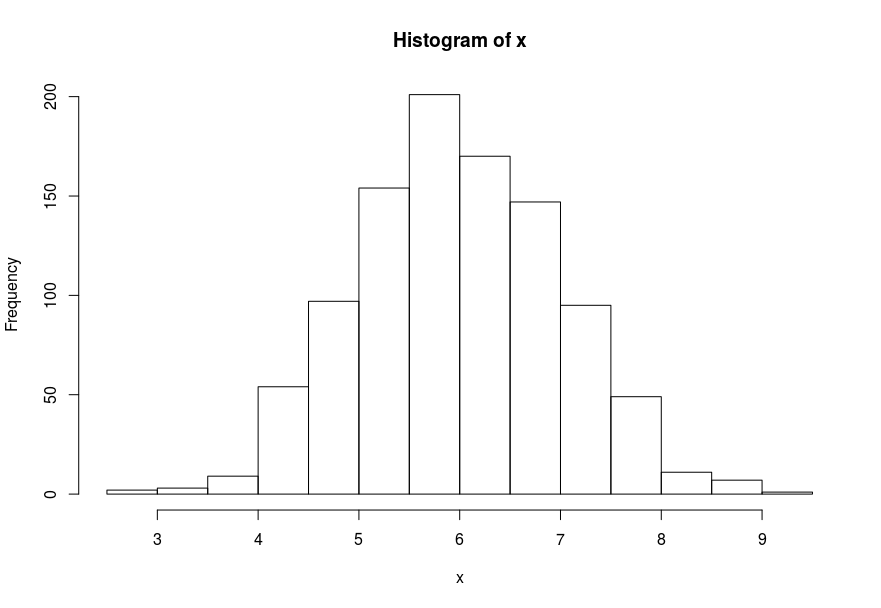
\includegraphics[width=\textwidth]{hist}
    \caption{Гистограмма времени подготовки
    к экзамену группы студентов}
\end{figure}

Каждому студенту с его временем подготовки
сопоставлен результат сдачи экзамена,
закодированный 0 или 1.
Чтобы сгенерированные данные имели
некоторую схожесть с реальностью,
нужно сделать, чтобы студенты,
которые затратили минимальное время по группе
на подготовку сдавали экзамен реже,
нежели студенты, которые уделили
наибольшее количество времени.
Для этой цели вводится коэффициент $\alpha$,
который показывает, какая часть с каждого
конца интервала времени будет порогом
точной несдачи и точной сдачи экзамена.
Для моделирования был выбран $\alpha = 0.3$,
т.е. 30\% студентов с наименьшим временем
не сдали экзамен и аналогично 30\%
с наибольшим сдали.
Оставшаяся средняя часть интервала
заполняется произвольно
из равномерного распределения.

\clearpage
\begin{figure}[H]
    \centering
    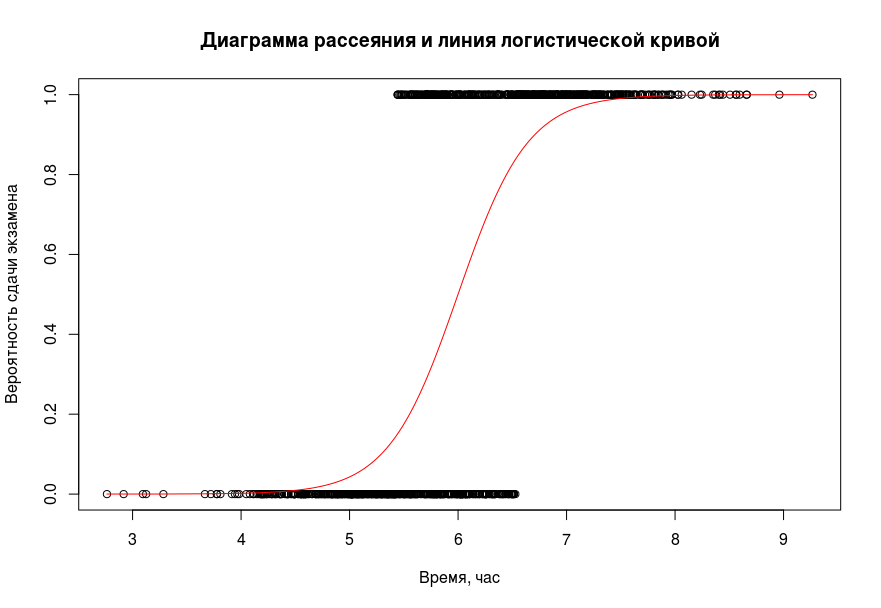
\includegraphics[width=\textwidth]{logit}
\end{figure}

На приведённом графике чёрными кружками
обозначены конкретные показатели времени,
красной линией показана логистическая кривая.

Вывод результатов построения логистической регрессии:

\lstinputlisting[lastline=23]{task.log}

Существует несколько способов
нахождения коэффициентов логистической регрессии.
В данном алгоритме они отыскиваются последовательно
с помощью итерационного метода наименьших квадратов
с использованием взвешивания элементов выборки.
Видно, что было произведено 6 итераций.

Свободный коэффициент равен $-18.6175$,
коэффициент при $x$ равен $3.1032$.
P-value значительном меньше 5\%,
можно сделать вывод,
что время подготовки к экзамену
значительно влияет на результат сдачи экзамена.

Можно построить 95\% доверительный интервал для найденных коэффициентов:

\lstinputlisting[firstline=25]{task.log}

\section*{Вывод}
Логистическая регрессия ---
полезный классический инструмент
для решения задачи регрессии.
С помощью логистической регрессии
можно оценивать вероятность того,
что событие наступит для конкретного испытуемого.

Линию логистической регрессии
можно рассматривать как функцию распределения.
Для данной смоделированной выборки
было замечено, что для сдачи экзамена
с 95\% достоверностью достаточно 7.72 часа из 10.

\section*{Исходный код}
Исходный код прилагается.

\end{document} % Конец документа
